\section{Theory and Algorithms}
\label{sec:theory}


\begin{figure}[hbt]
\centering
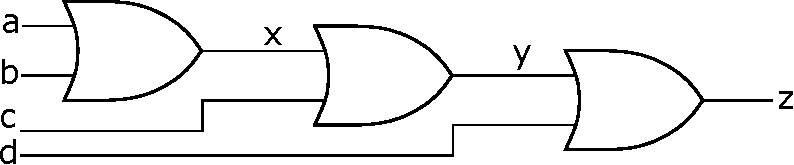
\includegraphics[scale=0.40]{Preliminaries-Theory/Chain_Or_Gates.pdf}
\caption{A chain of OR gates.}
\label{ChainOrGate}
\end{figure}

\begin{figure*}[hbt]
\centering
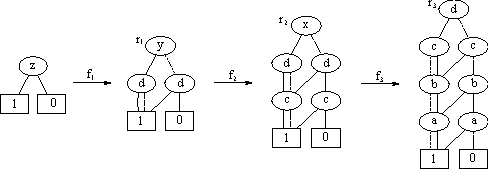
\includegraphics[scale=1.4]{./Preliminaries-Theory/red_steps.pdf}
\caption{Reduction of output of the circuit in Fig. \ref{ChainOrGate} by $f_1,f_2,f_3$.}
\label{red_steps}
\end{figure*}

Consider the circuit in Fig. \ref{ChainOrGate}, impose RTTO: {\it
  lex} term order with variable ordering as, $z>y>x>d>c>b>a$. The Boolean
polynomials for the circuit are: $f_1 = z + y\cdot d + y +d,
~f_2 = y + x\cdot c + x +c , ~f_3 = x + b\cdot a + b +a$.  Under RTTO,
$f_1, f_2, f_3$ forms a GB $G = \langle f_1,f_2,f_3 \rangle$. For verification, we have to reduce the
output $z$ modulo $G$. A classical symbolic algebra
 reduction using an explicit representation is carried out as: 

\begin{enumerate}
\item {\small $z \xrightarrow{f_1} y d +y +d$}
\item {\small $y d +y +d \xrightarrow{f_2} y + xdc + xd + dc + d \xrightarrow{f_2} xdc + xd + xc + x +dc + d + c$}
\item {\small $xdc + xd + xc + x +dc + d + c \xrightarrow{f_3} xd + xc + x  +
  dcba  + dcb + dca + dc + d + c \xrightarrow{f_3} xc + x + dcba +dcb
  + dca + dc + dba + db + da + d + c \xrightarrow{f_3} x  +dcba +dcb +
  dca + dc + dba + db + da + d + cba + cb + ca + c \xrightarrow{f_3}
  dcba +dcb + dca + dc + dba + db + da + d + cba + cb + ca + c + ba +
  b +a=r$}
\end{enumerate}


In the first step, $z$ is reduced by $f_1$ just {\it once} as that's the only term. In the
second step, the result of step one is reduced {\it twice} by $f_2$ as
the result has two terms containing variable $y$. Similarly,
{\it four} reductions by $f_3$ are required to 
reduce the result of step two into an expression containing only
primary inputs (which cannot be reduced further). 

{\it Observations:} i) Notice that the size of the final remainder 
corresponds to that of the worst case of a Boolean polynomial:
i.e. $r$ contains $2^n - 1\ (=15)$ monomial terms for $n\ (=4)$ variables. ii)
Classical division algorithms reduce the polynomials 1-step at a time,
where only one monomial is canceled in each step. iii) The number of
1-step reductions can increase exponentially as GBR progresses across
the circuit. 

It is clear that any data-structure that {\it explicitly} represents
each monomial will encounter space and time explosion: this includes
the dense-distributive representation of {\sc singular} computer
algebra tool \cite{DGPS}, or the ones used by
\cite{ciesielski:dac2015,rolf:date16}. The $F_4$-style
polynomial reduction of \cite{lv:tcad2013,pruss:tcad} simulates
division on a matrix $M$ representing the problem. However, each column
of $M$ corresponds to monomial generated in the division process,
therefore \cite{lv:tcad2013,pruss:tcad} also encounter this size
explosion. 

The use of ZBDDs can help overcome this explosion. Fig. \ref{red_steps} shows
the same reduction of $z$ by $f_1,f_2,f_3$ using ZBDDs (exact
procedure discussed later). The size of the ZBDDs after complete reduction by
$f_1,f_2,f_3$ increases linearly in the number of nodes. Subsequently, the final remainder has 
$2\cdot n - 1\ (=7)$ nodes (excluding the terminal 1 and 0 nodes) for $n\ (=4)$ variables.

%\begin{Proposition}
%For the worst case of the Boolean polynomial $F$ with $n$ variables and
%$2^n - 1$ monomials, the ZBDD representation of $F$ consists of
%$2\cdot n -1$ nodes in the graph.
%\end{Proposition}


{\bf ZBDD Representation:} %% We show how reduction is performed using
%% ZBDDs. 
% \subsection{ZBDD Representation}
The following steps describe the procedure for building ZBDDs for the polynomials of the gates of circuits.
\begin{enumerate}
	\item Obtain the RTTO for the variables (signals) of the circuits as $x_1 > x_2 > \dots > x_n$.
	\item Impose the same order on the ZBDDs.
	\item Declare ZBDDs for each of these variables.
	\item Use Eqn. (\ref{b2poly}) to model the gates of the circuit as Boolean polynomials. Build ZBDDs for
	these polynomials using the $+$ and $\cdot$ binary operations for modulo 2 sum and product of variables. The $+$
  operation can be implemented as $f+g = f \cup g - f \cap g$. However, in order to avoid the large intermediate 
  ZBDDs for the union we have implemented this operation as presented in Algorithm 1 in~\cite{polybori:2009}. 
	\item Traversing only the solid edges from the root node of a ZBDD to
  terminal {\bf 1} delivers the leading monomial of that polynomial.  
  The child node of the root at the solid edge's end will be 
  referred to as $then$ and the other child as $else$.
\end{enumerate} 

% The variable ordering imposed on the ZBDDs is the same as the one
% derived through RTTO. Then every path from the root to terminal {\bf
%   1} represents a monomial, with the 1-edge or solid-edge (resp. 0-edge or dotted-edge) denoting
% the presence (resp. absence) of the variable in the
% monomial. Traversing only the solid edges from the root node of a ZBDD to
% terminal {\bf 1} delivers the leading monomial $lm(f)$. The
% child node of the root at the solid edge's end will be referred to as $then$ and the other child as $else$. 

Once the ZBDDs for the circuit have been built and stored in $G$, we need to perform the reduction
$z_i \xrightarrow{G}_+r_i$ for each output bit $z_i$. The polynomial $r_i$ will be a canonical 
representation of $z_i$ in terms of primary inputs only. 

Consider  the step 2 of division corresponding to Fig. \ref{ChainOrGate}, where the
polynomial $r_1 = yd +y+d$ needs to be reduced by $f_2$. The ZBDDs for
$r_1$ and $f_2$ are shown in Fig. \ref{f2}. 
% The ZBDD for $r_1$ has
% three paths (corresponding to $yd,y,d$) terminating in the node 1 that
% correspond to its monomials.  
%The ZBDD manager creates the ZBDDs with the defined monomial order,
%and therefore, the topmost node in both ZBDDs is $f$. 
Checking if $lt(f_2)$ divides $lt(r_1)$ becomes trivial as we just
need to compare the indices (each variable has a unique index) of top-most nodes of ZBDDs 
for the polynomials $r_1$ and $f_2$, which in this case are equal.
Recall from Proposition~\ref{prop:top-order} that the $lt(f_i)$ of the polynomials for gates of the circuit will always be $x_i$. 
%(remember the leading monomial of $f_i$ is always a single variable due to RTTO).   


{\bf Division with ZBDDs: Cancel 1 monomial in every step}

The algorithm for conventional reduction procedure using ZBDDs is
shown in Algorithm~\ref{singlemon}. The input parameters are the ZBDD of the output bit 
of the circuit $z_i$ and $poly\_list$ containing the ZBDDs for 
the set of polynomials corresponding to the gates of the circuit. 
The algorithm is based on the classical division procedure (Algorithm~\ref{algo:mv_reduce}).
%The variables in the ZBDD manager are
%declared in the same order as the RTTO. For our example of
%Figure~\ref{ChainOrGate}, the first variable declared in the ZBDD
%manager is $z$, then $f$, and so on. 



%\vspace{-0.2in}
 Due to RTTO, the circuit polynomials for each gate are represented as $f_1= x_1 +
 else(f_1), \dots, f_s= x_s + else(f_s)$ with variable order 
 $x_1 > \cdots > x_s > \cdots > x_n$ (Prop. \ref{prop:top-order}). Note that the variables $\{x_{s+1}, \dots , x_{n}\}$ are 
 primary inputs and are not the output of any logic gate.  Then the elements
in $poly\_list$ are ordered $f_1 > f_2 > \dots > f_s$ $i.e.$ $poly\_list[1] = f_1, poly\_list[2] = f_2$ and so on. 
 Populating $poly\_list$ in this way avoids the search (Line 4, Algorithm~\ref{algo:mv_reduce}) required
 to find a polynomial $g \in poly\_list$ that can divide the leading
 term of $z_i$. While iterating over the polynomials $g \in poly\_list$
 if a certain polynomial does not divide the leading term of $z_i$, it
 will imply the polynomial is not in the logical cone of $z_i$.   

\begin{figure}[hbt]
\centering
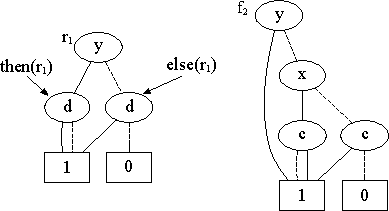
\includegraphics[scale=1]{Preliminaries-Theory/r1_f2.pdf}
\caption{ZBDDs for polynomial $r_1$ and $f_2$.}
\label{f2}
\end{figure}

%\vspace{-0.2in}
\begin{algorithm}
\caption{Reduction: Cancel 1 monomial every iteration}
\label{singlemon}
\begin{algorithmic}[1]
{\small
\Procedure{$single\_mon\_red$}{$z_i,poly\_list$}
\For{each $g \in poly\_list$}
\State $lead\_g = leading\_term(g)$
\State $lead\_z_i = leading\_term(z_i)$
\State $quotient = ZBDD\_Divide(lead\_z_i,lead\_g)$
\While{$quotient \neq zero$}
\State $prod = quotient \cdot g$
\State $z_i = z_i + prod$
\State $lead\_z_i = leading\_term(z_i)$
\State $quotient = ZBDD\_Divide(lead\_z_i,lead\_g)$
\EndWhile
\EndFor
\State \Return $z_i$
\EndProcedure
}
\end{algorithmic}
\end{algorithm}

The procedure $leading\_term(g)$ returns the leading term of 
the ZBDD representation of polynomial $g$. 
%The procedure starts at the root node and follows the THEN path until
%it reaches the terminal node 1. The cube of the variables, whose
%corresponding nodes are encountered on this path, gives us the
%leading term of the polynomial. 
If $g$ divides $f$, then the procedure $ZBDD\_Divide(f,g)$ (performs cube division) returns the quotient of the
division,  else it returns zero. Line 8 iteratively computes $z_i = z_i +
{lt(z_i) \over lt(g)}\cdot g$. The polynomial $z_i$ is completely reduced
$w.r.t.$ the polynomial $g$ in the while loop. 
% The $\cdot$ operator
% computes the product of two ZBDDs and the + operator is a modulo 2
% sum: $f + g = f \cup g - f \cap g$. 

\par {\bf Improved Reduction: Cancel multiple monomials in 1 step:}
Next, we will show how $z_i$ can be reduced by a polynomial $g$ {in one step}. In the 
example of Fig.~\ref{red_steps}, the primary output $z$ is reduced by $f_1$ to get $r_1$. The next  step 
is to reduce $r_1$ by $f_2$ to get $r_2$. To demonstrate our
approach we will show how the reduction of $r_1$ by $f_2$ can be achieved in one step.
%There are two monomials in $r_1$ that contain $y$, namely $yd, y$. Both can be canceled by $lt(f_2) = f$ in one step,
%eliminating the need of the while loop in Algorithm~\ref{singlemon}.   
\par The polynomial $r_1 = yd + y + d$ can be written as $y\cdot(d+1) + d$. If we perform 1-step reduction of $r_1$ by $f_2$ we get
the quotient $d+1$. This quotient is visible as the polynomial 
represented by the $then$-node of $r_1$ (Fig. \ref{f2}). 
So the reduction can be performed by
multiplying $d + 1$ with $f_2$ and adding this 
product to $r_1$ $\pmod{2}$:
% \vspace{-0.1in}
%{\small
\begin{align*}
& (yd + y + d) + (d + 1)\cdot(y + xc + x + c) \pmod{2}\\
&= 2\cdot(yd + y) + d + (d+1)\cdot(xc + x + c) \pmod{2}\\
&= d + (d+1)\cdot(xc + x + c)  \pmod{2}
\end{align*}
%\vspace{-0.1in}
%Use the follwing notation
%\begin{align*}
%& \text{$head(R_1)$ = 1-branch (THEN) of top-most node of $R_1$} = d + 1,\\
%& \text{$tail(R_1)$ = 0-branch (ELSE) of top-most node of $R_1$} = d,\\
%& \text{$head(P)$ = 1-branch of top-most node of $P$} = f,\\
%& \text{$tail(P)$ = 0-branch of top-most node of $P$} = ec + e + c.
%\end{align*}
%}
Notice that $else(r_1)=d$ and $else(f_2)=xc+x+c$. In addition, we know that $2\cdot(fd + f) \pmod{2}$ is going
to be zero. Therefore, in order to reduce number of operations, we
directly use the last step as a formula for reduction: 
%\vspace{-0.05in}
%{\small
\begin{align*}
r_1 \xrightarrow{f_2}_+&= d + (d+1)\cdot(xc + x + c) \\
& else(r_1) + then(r_1)\cdot else(f_2)
\end{align*}
% }%
So the reduction process effectively involves just two operations, a
modulo 2 sum and a product. {\it This has the effect of canceling all
  the terms in $r_1$ that can be canceled by $lt(f_2)$ in one-go,
  implicitly canceling multiple monomials in one step}.  

The algorithm for Multiple Monomial Reduction is shown in
Algorithm~\ref{multimon}, where the notations, $z_i$ and $poly\_list$,
are same as in Algorithm \ref{singlemon}. Unlike in
Algorithm~\ref{singlemon}, however, where we need to find the quotient of
$lead\_z_i/lead\_g$, Algorithm~\ref{multimon} only determines if
$lead\_g$ can divide $z_i$ at all (in this case the quotient is
$then(z_i)$). This can be accomplished by just comparing the indices of
top-most nodes of $z_i$ and $g$. This algorithm significantly reduces
the number of iterations, which now exactly equals the size of
$poly\_list$. For the example of Fig. \ref{ChainOrGate}, the number
of iterations is 3 using Algorithm~\ref{multimon}, whereas 7
iterations are required using Algorithm \ref{singlemon}. 

\begin{algorithm}
\caption{Reduction: Cancel multiple monomials}
\label{multimon}
\begin{algorithmic}[1]
{\small
\Procedure{$multi\_mon\_red$}{$z,poly\_list$}
\For{each $g \in poly\_list$}
%\State $G_i = POLY\_LIST[i]$
%\State $index_{G_i} = G_i \rightarrow index$
%\State $index_F = F \rightarrow index$

\If{ $index(g) == index(z)$} 
%\State $p_1 = then(f)$
%\State $p_2$ = else(f)
%\State tail = else($g_i$)
%\State prod = $p_1$ $ \cdot$  tail
\State $z = else(z) + then(z)\cdot else(g)$
\EndIf

\EndFor
\State \Return $z$
\EndProcedure
}
\end{algorithmic}
\end{algorithm}



We have implemented the above GBR procedures directly using the CUDD
package~\cite{cudd}. The circuit under verification is analyzed, RTTO based
variable order is imposed on the ZBDDs, and the Boolean polynomials of
the circuit are represented as unate cube sets. 
The polynomials of of the gates of circuit, $f_i \in G$, are
inserted in $poly\_list$ according to the variable order $x_1 > \dots
> x_i > \dots > x_n$, where $f_i = x_i + else(f_i)$ (this is due to
Prop. \ref{prop:top-order}). To perform GBR $z_i\xrightarrow{G}_+ r_i$
Algorithm \ref{multimon} is invoked to obtain the remainder. 
%The division algorithm in {\sc
%  polybori} \cite{polybori} is conceptually similar to that of
%Algorithm 1, whereas Algorithm 2 is our main contribution.
